\documentclass[12pt, a4paper]{article}
\usepackage[spanish]{babel}
\usepackage[utf8]{inputenc}
\usepackage{graphicx}
\usepackage{geometry}
\usepackage{fancyhdr}
\usepackage{float}
\usepackage{titling}
\usepackage{hyperref}
\usepackage{url}

% Márgenes
\geometry{a4paper, margin=2.5cm}

% Encabezado y pie de página
\pagestyle{fancy}
\fancyhf{}
\rhead{
\includegraphics[height=1.2cm]{images/logo-usm.png}} % <-- Cambia si usas otro logo
\lhead{Grupo 19\\ Visualización de Datos}
\setlength{\headheight}{20pt}
\setlength{\headsep}{1cm}
\rfoot{Página \thepage}

% Configuración del logo en portada
\pretitle{
  \begin{center}
  \vspace{1cm}
  
\includegraphics[width=0.5\textwidth]{images/logo-usm.png}\\ % <-- Cambia si usas otro logo
  \vspace{1.5cm}
  \LARGE
}
\posttitle{\end{center}}

% Título del informe
\title{Ciberseguridad y Ataques cibernéticos}
\author{Felipe Campaña, Javier Gómez, Matias Elgueta}
\date{\today\\[2cm]}

\begin{document}
\maketitle

% ---------------------------------------------------------------------------------
\vspace*{0.3cm}
\begin{figure}[H]
    \centering
    \begin{minipage}[t]{0.45\linewidth}
    \end{minipage}
    \hfill
    \begin{minipage}[t]{0.45\linewidth}
    \end{minipage}
\end{figure}

\section*{Trabajo en grupo}

\subsection*{Enlace al dataset}
\url{https://cissm.umd.edu/cyber-events-database}

\vspace{1em}
\subsection*{Mapa 1: Clasificación de tipos de ciberataques por país (Flourish)}

\begin{figure}[H]
    \centering
    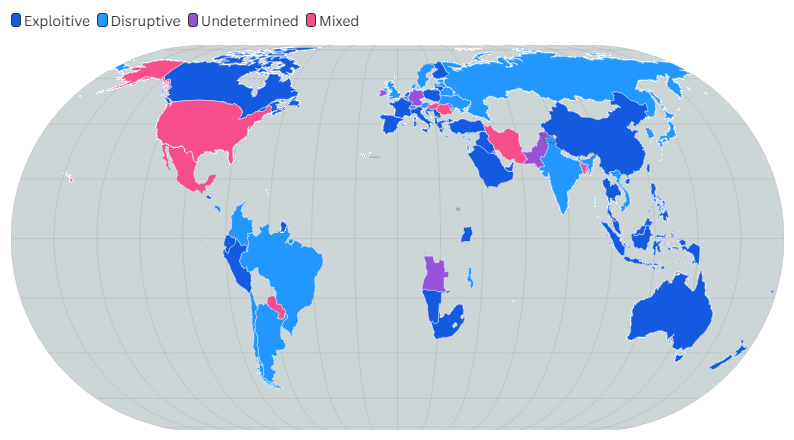
\includegraphics[width=0.95\textwidth]{images/punto_cate.png}
    \caption{Clasificación de ciberataques según tipo de evento por país. Fuente: Elaboración propia con datos.}
\end{figure}

\textbf{Tipo de mapa:} Mapa de puntos categorizados \\
\textbf{Ubicación en el espectro de mapas:} Cualitativo – Representación nominal de eventos clasificados. \\

\textbf{Esquemática:} \\
\begin{itemize}
    \item \textit{Descripción:} Cada punto representa un país y está coloreado según el tipo predominante de ciberataque recibido (\textit{Exploitive}, \textit{Disruptive}, \textit{Mixed}, \textit{Undetermined}).
    \item \textit{Secuencia:} Se utilizó un dataset con información sobre actores, motivos y eventos de ciberataques. Los datos fueron agrupados por país y se extrajo el tipo de evento más frecuente para representarlo visualmente mediante Flourish.
\end{itemize}

\textbf{Colores utilizados:} \\
Paleta distintiva por categoría nominal. Cada color representa un tipo de ataque, facilitando la comparación entre países. Se utilizó contraste alto para mejorar la diferenciación visual entre clases.

\textbf{Tipografía empleada:} \\
Flourish aplica una tipografía sans-serif moderna, clara y centrada en la legibilidad, compatible con visualizaciones web interactivas.

\textbf{Objetivo del mapa:} \\
Identificar y comparar el tipo de ciberataque más frecuente en cada país, para comprender patrones globales y regionales de amenazas.



\subsection*{Mapa 2: Mapa de Calor de Ciberataques por País (CARTO)}

\begin{figure}[H]
    \centering
    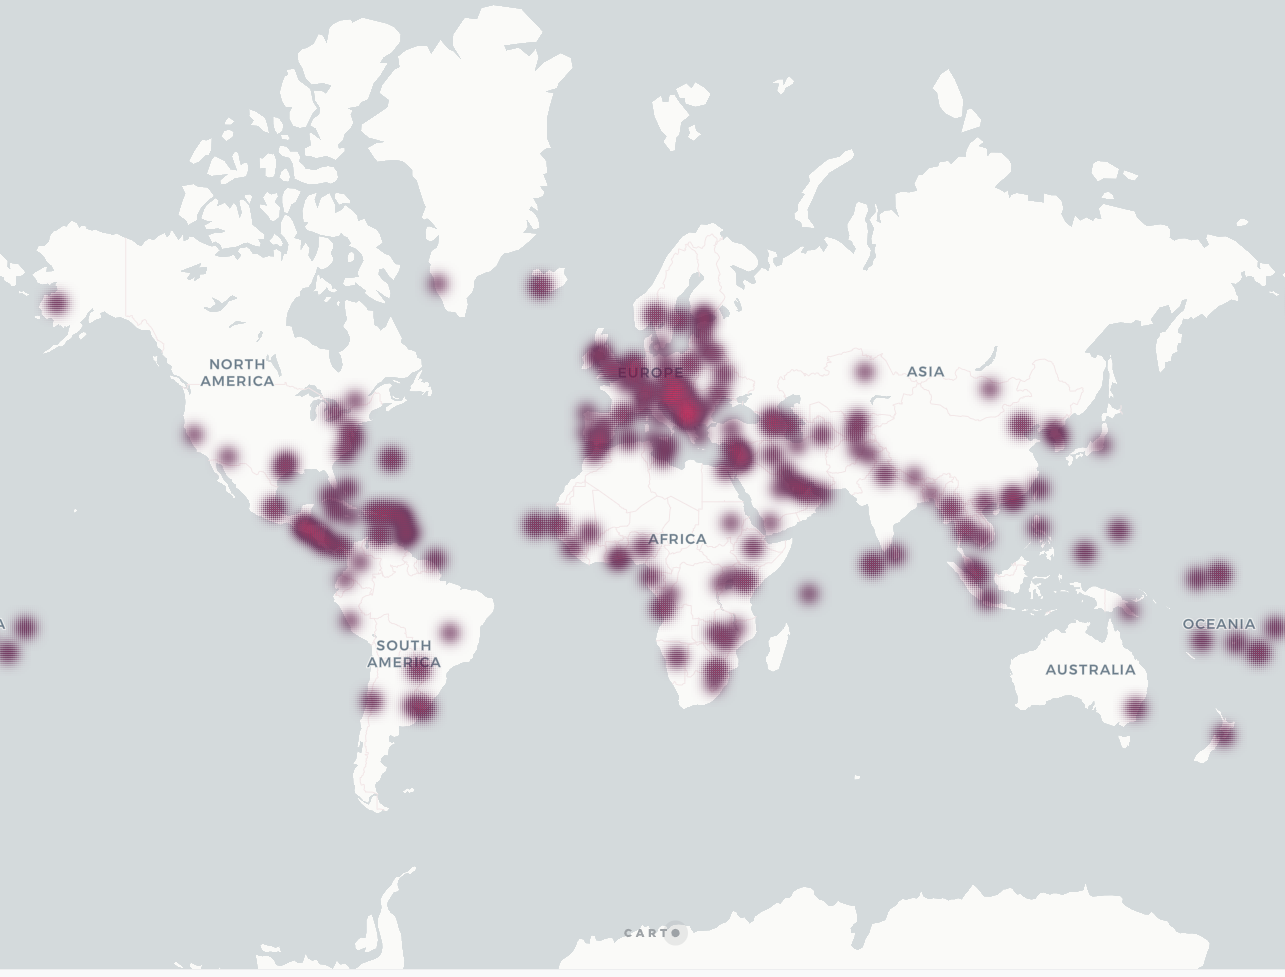
\includegraphics[width=0.95\textwidth]{images/Mapa_calor_FC.png}
    \caption[1]{Fuente: \url{https://clausa.app.carto.com/map/f16b7877-40d4-4182-8c3e-043b5bdb2aa2}}
\end{figure}

\textbf{Tipo de mapa:} Mapa de calor (heatmap) \\
\textbf{Ubicación en el espectro de mapas:} Cuantitativo – Distribución espacial de densidad por unidad política (país). \\

\textbf{Esquemática:} \\
\begin{itemize}
    \item \textit{Descripción:} Visualización de la concentración de incidentes cibernéticos registrados entre 2014 y 2024 por país.
    \item \textit{Secuencia:} Se partió desde el dataset completo, se agrupó por país y se contó la cantidad de incidentes. Se añadieron coordenadas geográficas y se cargó el resultado a CARTO como mapa de calor.
\end{itemize}

\textbf{Colores utilizados:} \\
Se utilizó una paleta monocromática que va desde blanco a rojo oscuro. Esta elección refuerza la percepción de urgencia y riesgo en zonas con alta concentración de incidentes.

\textbf{Tipografía empleada:} \\
CARTO emplea una tipografía sans-serif clara, de alto contraste, que mantiene coherencia con el diseño minimalista de la plataforma. Esto permite que el foco esté en los datos visualizados y no en elementos distractores.



\vspace{1em}
\subsection*{Mapa 3: Flujos de ciberataques entre países (Kepler.gl)}

\begin{figure}[H]
    \centering
    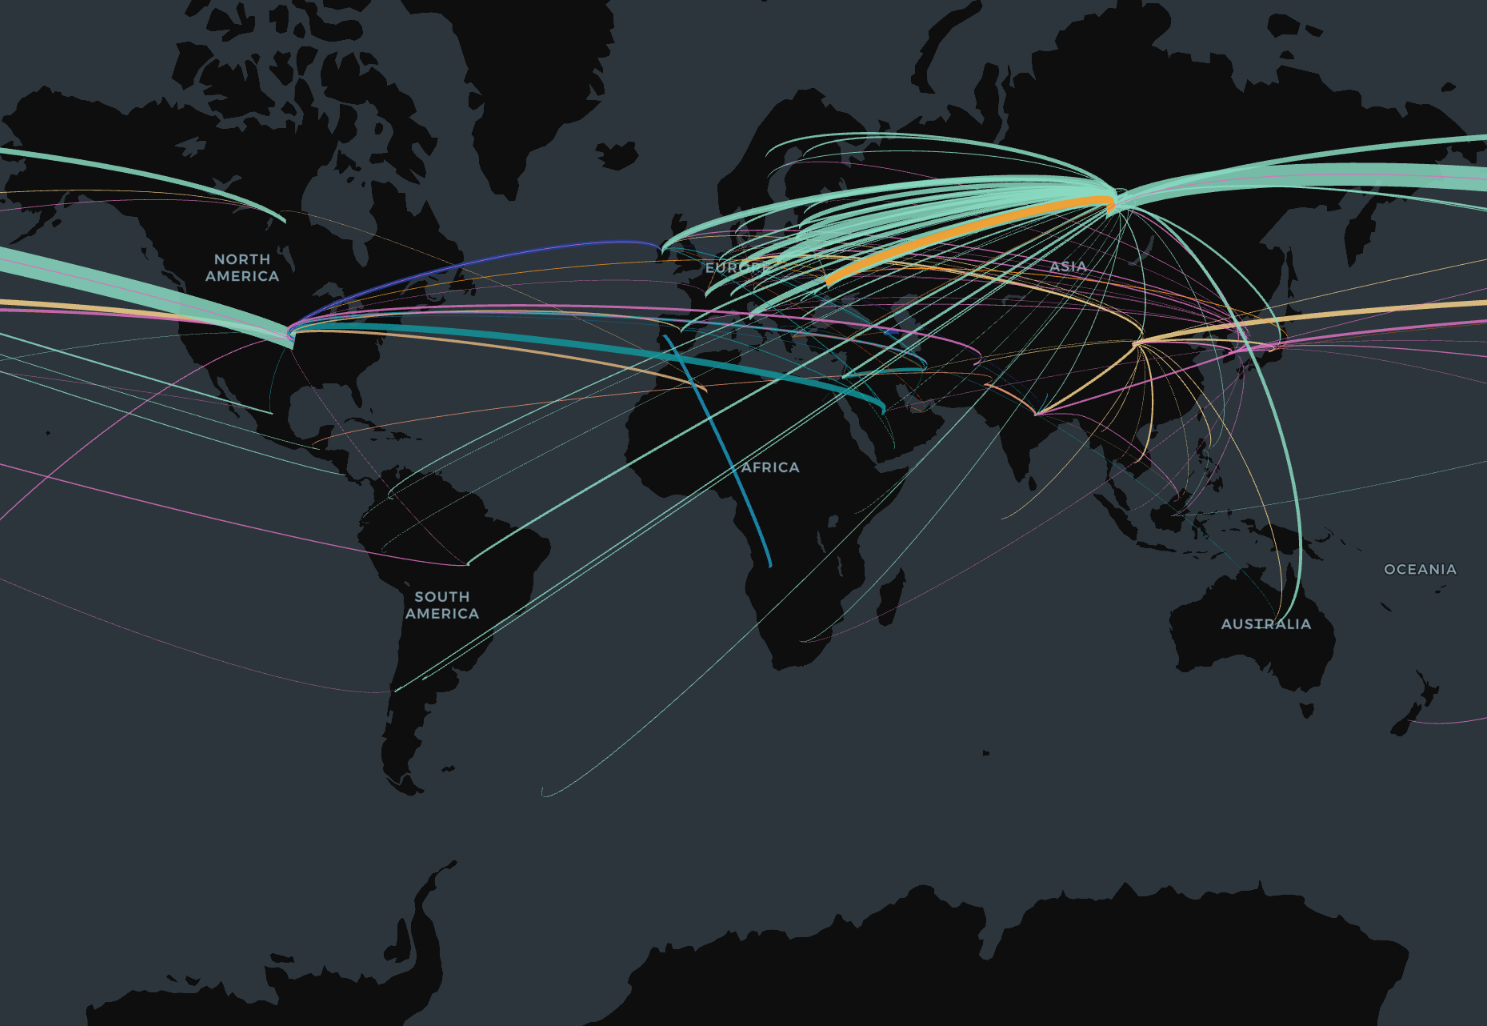
\includegraphics[width=0.95\textwidth]{images/Arc_Layer.png}
    \caption{Flujos de ciberataques entre países. Fuente: Elaboración propia en plataforma Kepler.gl. \url{https://kepler.gl/demo/map?mapUrl=https://dl.dropboxusercontent.com/scl/fi/gaxz7hj5uuyfrv5h2ljph/keplergl_qn6or6.json?rlkey=75daex9obuvd2m11ey8nxoiw4&dl=0}}
\end{figure}

\textbf{Tipo de mapa:} Mapa de flujos (Arc Layer) \\
\textbf{Ubicación en el espectro de mapas:} Exploratorio + Relacional-cuantitativo / Presentacional. \\

\textbf{Esquemática:} \\
\begin{itemize}
    \item \textit{Descripción:} 
        \begin{itemize}
            \item \textit{Origen (actor): } Punto inicial del arco.
            \item \textit{Destino (víctima): } Punto final.
            \item \textit{Grosor : } Numero de ataques.
            \item \textit{Color : } Distingue al país origen (paleta multicromática).
        \end{itemize}
    \item \textit{Secuencia:} Utilizando el dataset original se genero un dataset secundario que registra el numero de ataques registrados (actor country, victim country, attacks), Se añadieron cordenadas geograficas a cada fila de este dataset generando un dataset final el cual se subio a la plataforma \textit{Kepler.gl} para generar el Mapa de Flujos.
\end{itemize}

\textbf{Colores utilizados:} \\
Paleta de diez matices suaves (cian, violeta, aqua, amarillo-verdoso, rosa, etc.) aplicados a los arcos; mantiene contraste sobre fondo Dark (\#111b25 aprox.) de Kepler.
Justificación: colores diferenciados ayudan a reconocer rápidamente países origen sin recargar; fondo oscuro hace resaltar las líneas y reduce distracción.

\textbf{Tipografía empleada:} \\
En Kepler, se utiliza la fuente sans-serif por defecto (Inter/Roboto).

\textbf{Objetivo del mapa:} \\
Dirigido a analistas de ciberseguridad, periodistas de datos y responsables de política pública para detectar hubs emisores de amenazas, rutas de ataque recurrentes y posibles brechas de defensa a nivel global.

% ===================== INTEGRANTE 1 =====================
\section*{Análisis por Integrante}

\subsection*{Integrante 1: Javier Gomez}


\subsubsection*{Gráfico 1: Mapa de puntos categorizados}
\begin{figure}[H]
    \centering
    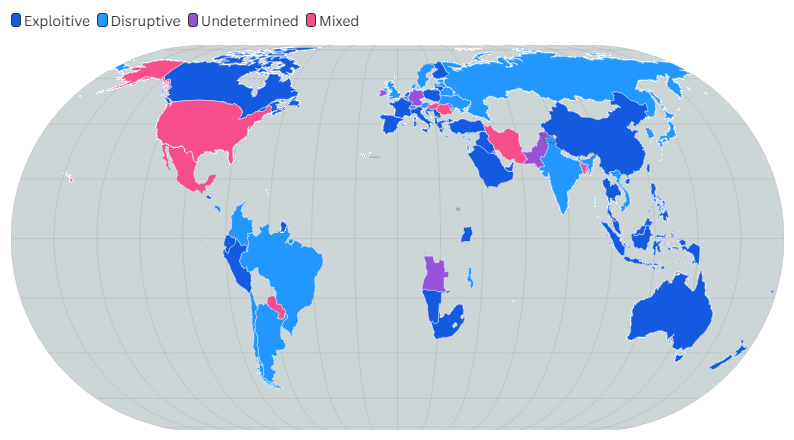
\includegraphics[width=0.9\textwidth]{images/punto_cate.png}
    \caption{Fuente: Elaboración propia con datos}
\end{figure}

\paragraph{Descripción cualitativa del dataset:}

El conjunto de datos contiene información sobre ataques cibernéticos dirigidos a diferentes países. Cada registro describe:
\begin{itemize}
    \item El tipo de actor que realiza el ataque (por ejemplo, \textit{Nation-State}, \textit{Criminal}).
    \item El motivo del ataque (\textit{Sabotage}, \textit{Financial}, etc.).
    \item El tipo de evento (\textit{Exploitive}, \textit{Disruptive}, etc.).
    \item El país objetivo del ataque.
\end{itemize}
Esta información permite clasificar a los países según el tipo de ataque más común que han recibido, representado gráficamente en el mapa mediante distintos colores.

\paragraph{Objetivo de la visualización:}

\begin{itemize}
    \item \textbf{¿Qué pregunta busca responder?} \\
    ¿Qué tipo de ataques cibernéticos predominan en cada país y cómo se distribuyen globalmente?

    \item \textbf{¿A qué público está dirigida?} \\
    A responsables de ciberseguridad, analistas de riesgos, académicos y tomadores de decisiones en políticas públicas.

    \item \textbf{¿Qué acción o decisión podría apoyar?} \\
    Esta visualización puede ayudar a:
    \begin{itemize}
        \item Identificar patrones geográficos de ciberataques.
        \item Establecer prioridades de protección en función del tipo de amenaza.
        \item Fomentar cooperación internacional en ciberseguridad.
    \end{itemize}
\end{itemize}

\paragraph{Conclusiones:}
\begin{itemize}
    \item La mayoría de los países presentan ataques del tipo \textbf{Exploitive}, lo que indica una tendencia a aprovechar vulnerabilidades sin necesariamente causar interrupciones.
    \item Algunos países, como Estados Unidos, muestran una predominancia de ataques \textbf{Disruptive}, que buscan causar interrupciones o daños visibles.
    \item Aparecen categorías \textbf{Mixed} o \textbf{Undetermined} en países donde hay múltiples tipos de ataques o falta de información clara.
    \item Existe una correlación geopolítica: regiones con conflictos o tensiones políticas muestran ataques más agresivos o frecuentes, como en el caso de Ucrania e Irán.
\end{itemize}
\subsubsection*{Anexo: Ataques saboteadores por actores estatales}
\begin{figure}[H]
    \centering
    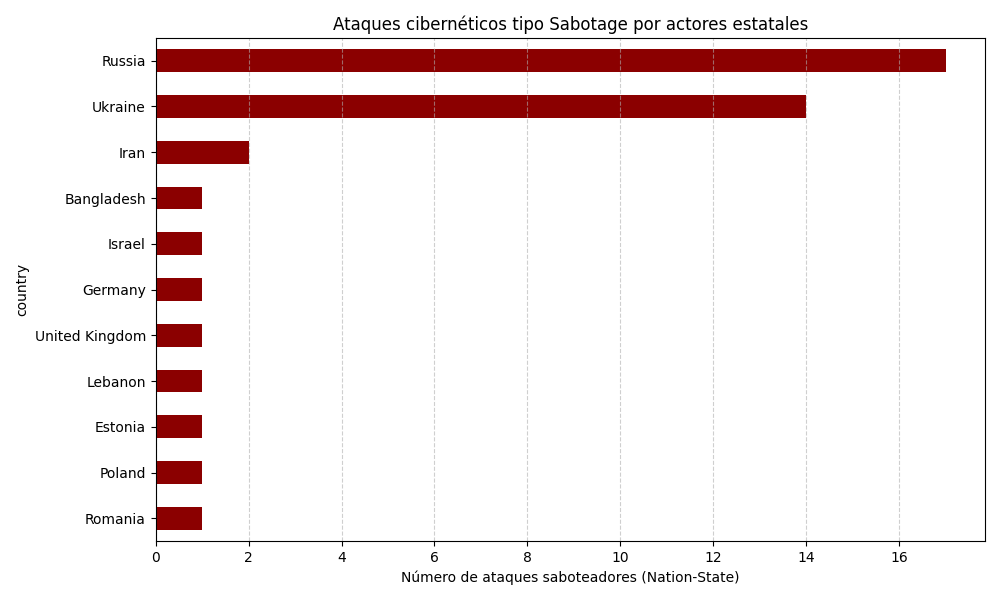
\includegraphics[width=0.8\textwidth]{images/sabotage_state.png}
    \caption{Ataques cibernéticos con motivo de sabotaje realizados por actores estatales. Fuente: Elaboración propia con datos del dataset.}
\end{figure}



% ===================== INTEGRANTE 2 =====================
\newpage
\subsection*{Integrante 2: Felipe Campaña}

\subsubsection*{Mapa 2: [Mapa de Calor en CARTO]}
\begin{figure}[H]
    \centering
    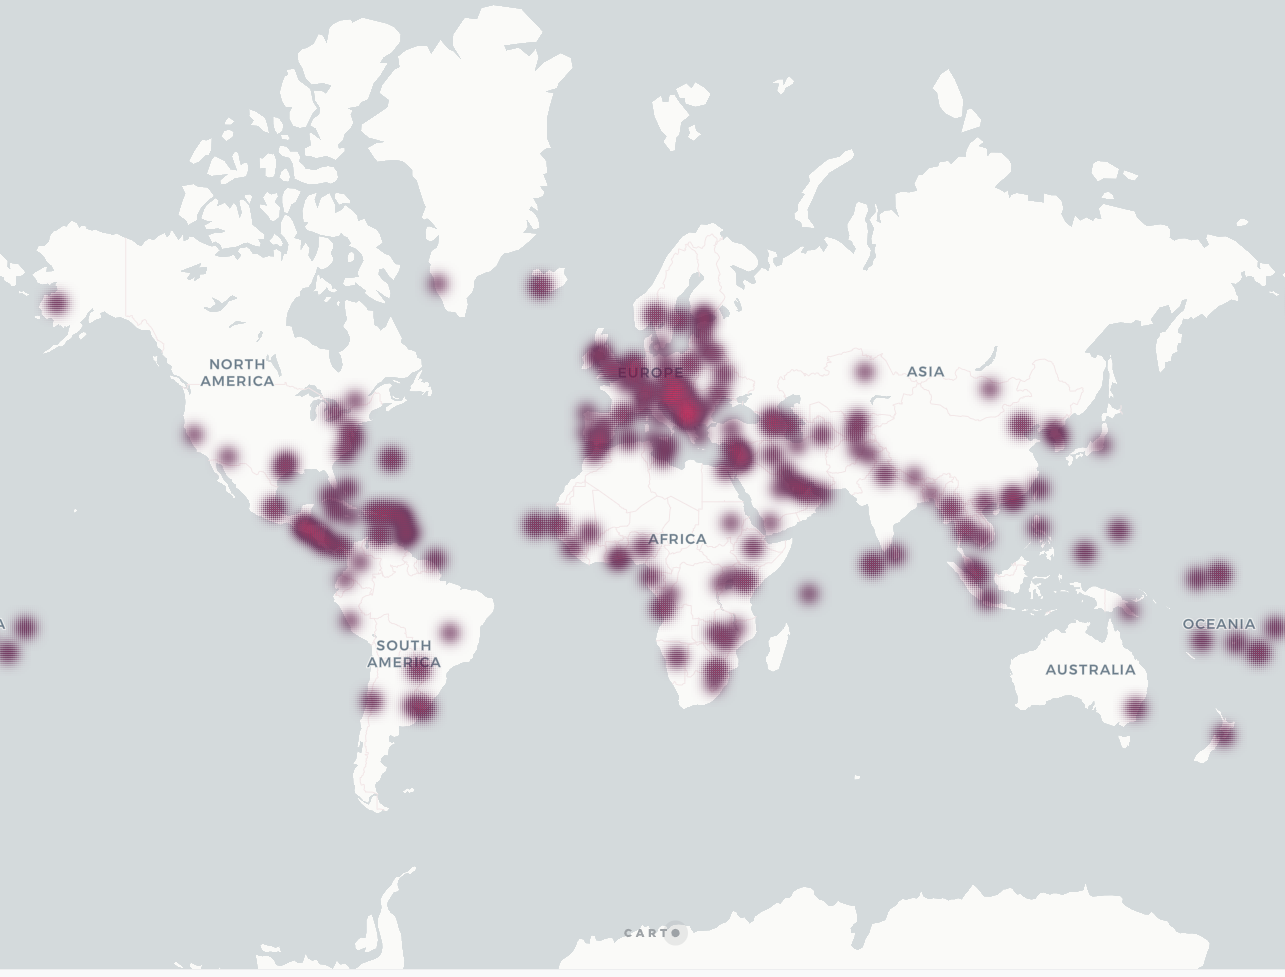
\includegraphics[width=0.85\textwidth]{images/Mapa_calor_FC.png}
    \caption[1]{Fuente: \url{https://clausa.app.carto.com/map/f16b7877-40d4-4182-8c3e-043b5bdb2aa2}}
\end{figure}

\textbf{Descripción cualitativa del dataset:} \\
El dataset utilizado proviene de la base de datos \textit{Cyber Events Database (2014–2024)} de la Universidad de Maryland. Esta base documenta más de 14.000 eventos de ciberseguridad relevantes a nivel mundial, incluyendo país afectado, tipo de ataque, actor responsable, sector y fecha. Se procesó agrupando los datos por país víctima para contar la cantidad de incidentes por ubicación geográfica.

\vspace{0.5em}
\textbf{Objetivo de la visualización:} \\
\begin{itemize}
    \item \textit{¿Qué pregunta busca responder?} \\
    ¿En qué países se han concentrado más ciberataques registrados entre 2014 y 2024?
    
    \item \textit{¿A qué público está dirigida?} \\
    Principalmente a periodistas de datos, investigadores en ciberseguridad y tomadores de decisiones en políticas públicas tecnológicas.

    \item \textit{¿Qué acción o decisión podría apoyar?} \\
    Esta visualización permite identificar regiones con alta exposición a amenazas cibernéticas, ayudando a priorizar recursos en ciberdefensa, programas de concientización o cooperación internacional.
\end{itemize}

\vspace{0.5em}
\textbf{Tipo de visualización:} \\
Mapa de calor (\textit{Heatmap}) realizado con la plataforma CARTO. Representa la densidad de incidentes cibernéticos según país. Mientras más rojo concentrado, mayor es la cantidad de eventos registrados en esa región.

\vspace{0.5em}
\textbf{Justificación de diseño:} \\
\begin{itemize}
    \item \textbf{Colores:} Se utilizó una escala monocromática rojo oscuro $\rightarrow$ blanco. El rojo transmite alerta, urgencia y riesgo, reforzando el mensaje de amenaza.
    \item \textbf{Tipografía y estilo:} CARTO aplica tipografía clara sin ruido visual. Se privilegia la lectura del mapa más que el texto.
    \item \textbf{Geocodificación:} Se asignaron coordenadas geográficas centrales a cada país para representar los datos en el mapa.
\end{itemize}

\vspace{0.5em}
\textbf{Conclusiones del gráfico:} \\
\begin{itemize}
    \item América del Norte, Europa Occidental y partes de Asia (China, Corea del Sur, India) son focos principales de ciberataques.
    \item Hay una notable concentración en países desarrollados, lo que puede asociarse tanto a mayor exposición tecnológica como a mejor capacidad de reporte.
    \item Regiones como África y Oceanía muestran baja densidad, aunque esto puede deberse a subregistro o menor cobertura mediática.
    \item El mapa permite hacer inferencias sobre la correlación entre infraestructura digital y volumen de ciberincidentes.
\end{itemize}

% ===================== INTEGRANTE 3 =====================
\newpage
\subsection*{Integrante 1: Matías Elgueta}

\subsection*{Mapa 3: Flujos de ciberataques entre países (Kepler.gl)}

\begin{figure}[H]
    \centering
    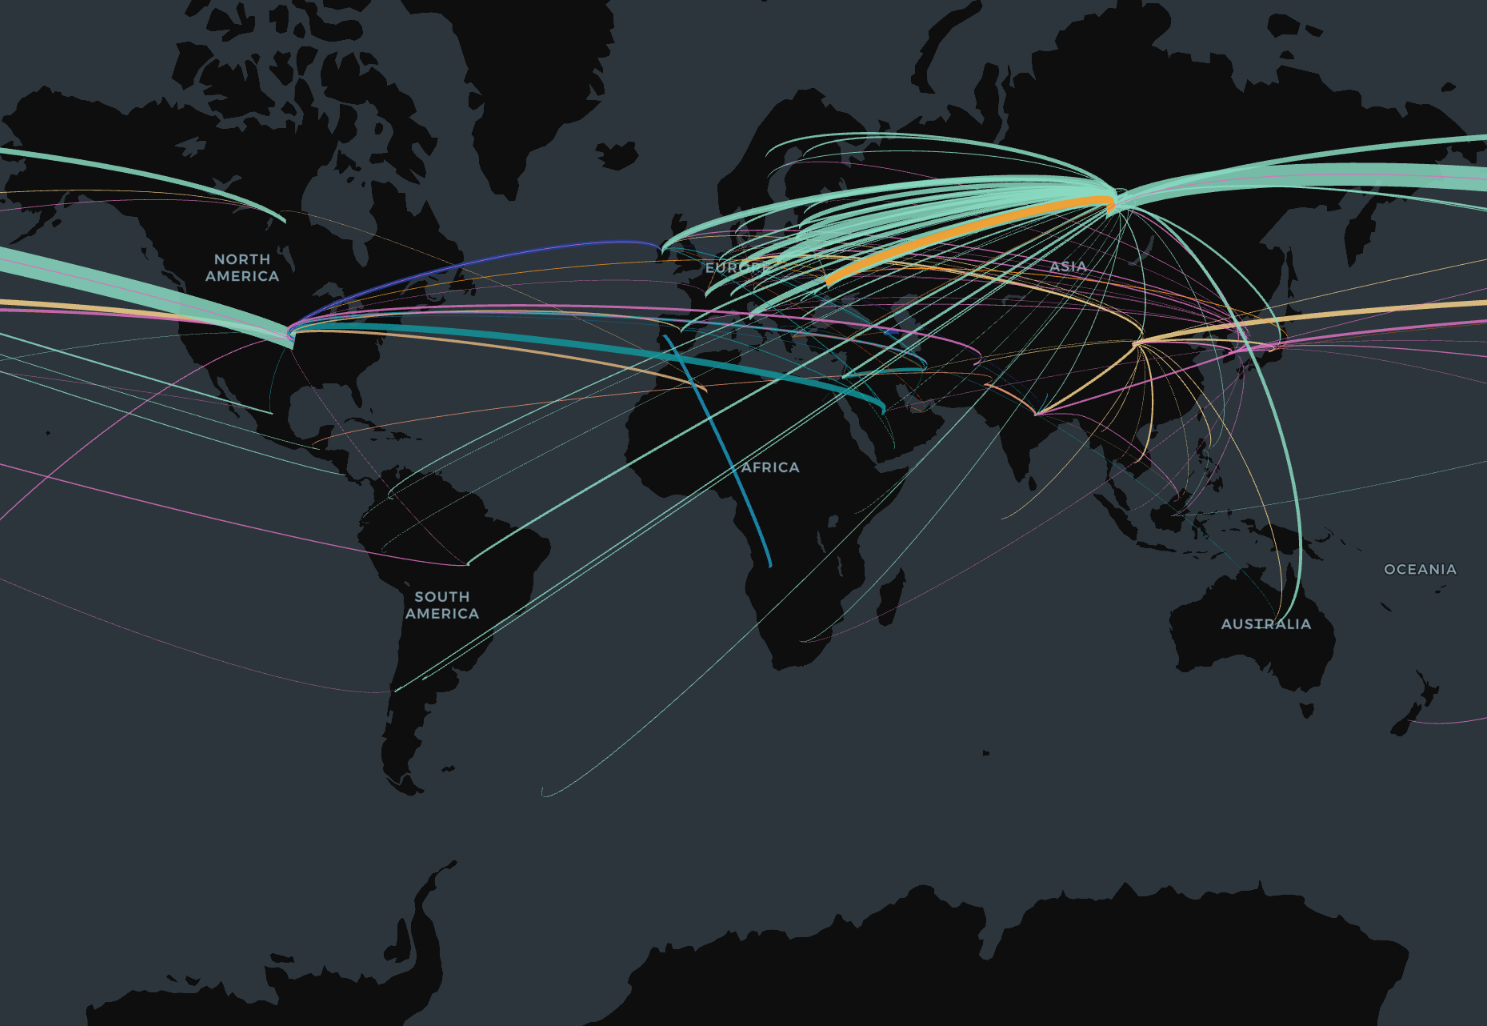
\includegraphics[width=0.95\textwidth]{images/Arc_Layer.png}
    \caption{Flujos de ciberataques entre países. Fuente: Elaboración propia en plataforma Kepler.gl. \url{https://kepler.gl/demo/map?mapUrl=https://dl.dropboxusercontent.com/scl/fi/gaxz7hj5uuyfrv5h2ljph/keplergl_qn6or6.json?rlkey=75daex9obuvd2m11ey8nxoiw4&dl=0}}
\end{figure}

\paragraph{Descripción cualitativa del dataset:}

El dataset utilizado contiene información agregada sobre ciberataques internacionales ocurridos entre 2014 y 2024. Representa relaciones entre países en función de la cantidad de ataques registrados desde un país atacante hacia uno víctima.
Se trata de un dataset relacional y espacial, útil para identificar patrones de conectividad, flujos de agresión digital y concentraciones geográficas de actividad ofensiva en el ciberespacio.

\paragraph{Objetivo de la visualización:}

\begin{itemize}
    \item \textbf{¿Qué pregunta busca responder?:} \\
    \textit{¿Qué países atacan a cuáles?} El mapa busca revelar los principales emisores y receptores de ciberataques a nivel internacional, así como la dirección e intensidad de estos flujos.

    \item \textbf{¿A qué público está dirigida?} \\
    A analistas de ciberseguridad, periodistas de datos y tomadores de decisiones en política digital o relaciones internacionales. También es útil para el público general interesado en la dimensión geopolítica de los ciberataques.

    \item \textbf{¿Qué acción o decisión podría apoyar?} \\
    Apoya la identificación de amenazas internacionales y la priorización de estrategias defensivas. También puede orientar decisiones diplomáticas, inversiones en ciberdefensa y campañas de concientización regionalizadas según patrones observados.

\paragraph{Conclusiones:}
\begin{itemize}
    \item \textbf{Rusia destaca como principal origen de ciberataques.}
    Se observa una gran concentración de líneas gruesas saliendo desde su territorio, lo que indica una alta actividad ofensiva hacia múltiples regiones del mundo.
    \item \textbf{Estados Unidos es el país más atacado.}
    Es el punto de llegada de los arcos más gruesos del mapa, especialmente desde Rusia, lo que lo posiciona como el principal objetivo de ataques internacionales.
    \item \textbf{Conflictos regionales como el de Rusia–Ucrania también son visibles.}
    Se evidencian flujos visibles en ambos sentidos entre estos países, mostrando un intercambio constante de ataques, destacando la dimensión digital del conflicto geopolítico.
    \item {Europa oriental y Asia son zonas de alta densidad de flujos.}
    Estas regiones presentan múltiples líneas cruzadas y agrupadas, lo que sugiere que son zonas estratégicas tanto como origen como destino de ciberataques.

\end{itemize}


\textbf{Repositorio:}  
\label{anexo:repositorio}

Acceso al repositorio en el siguiente link:  
\url{https://github.com/usuario/repositorio.git}

\end{document}
